\section{Architecture}

To start, the code implementation can be accessed at \url{https://github.com/pranay-bh/helm-keycloak} for complete architectural setup.


\begin{figure}[ht]
    \centering
    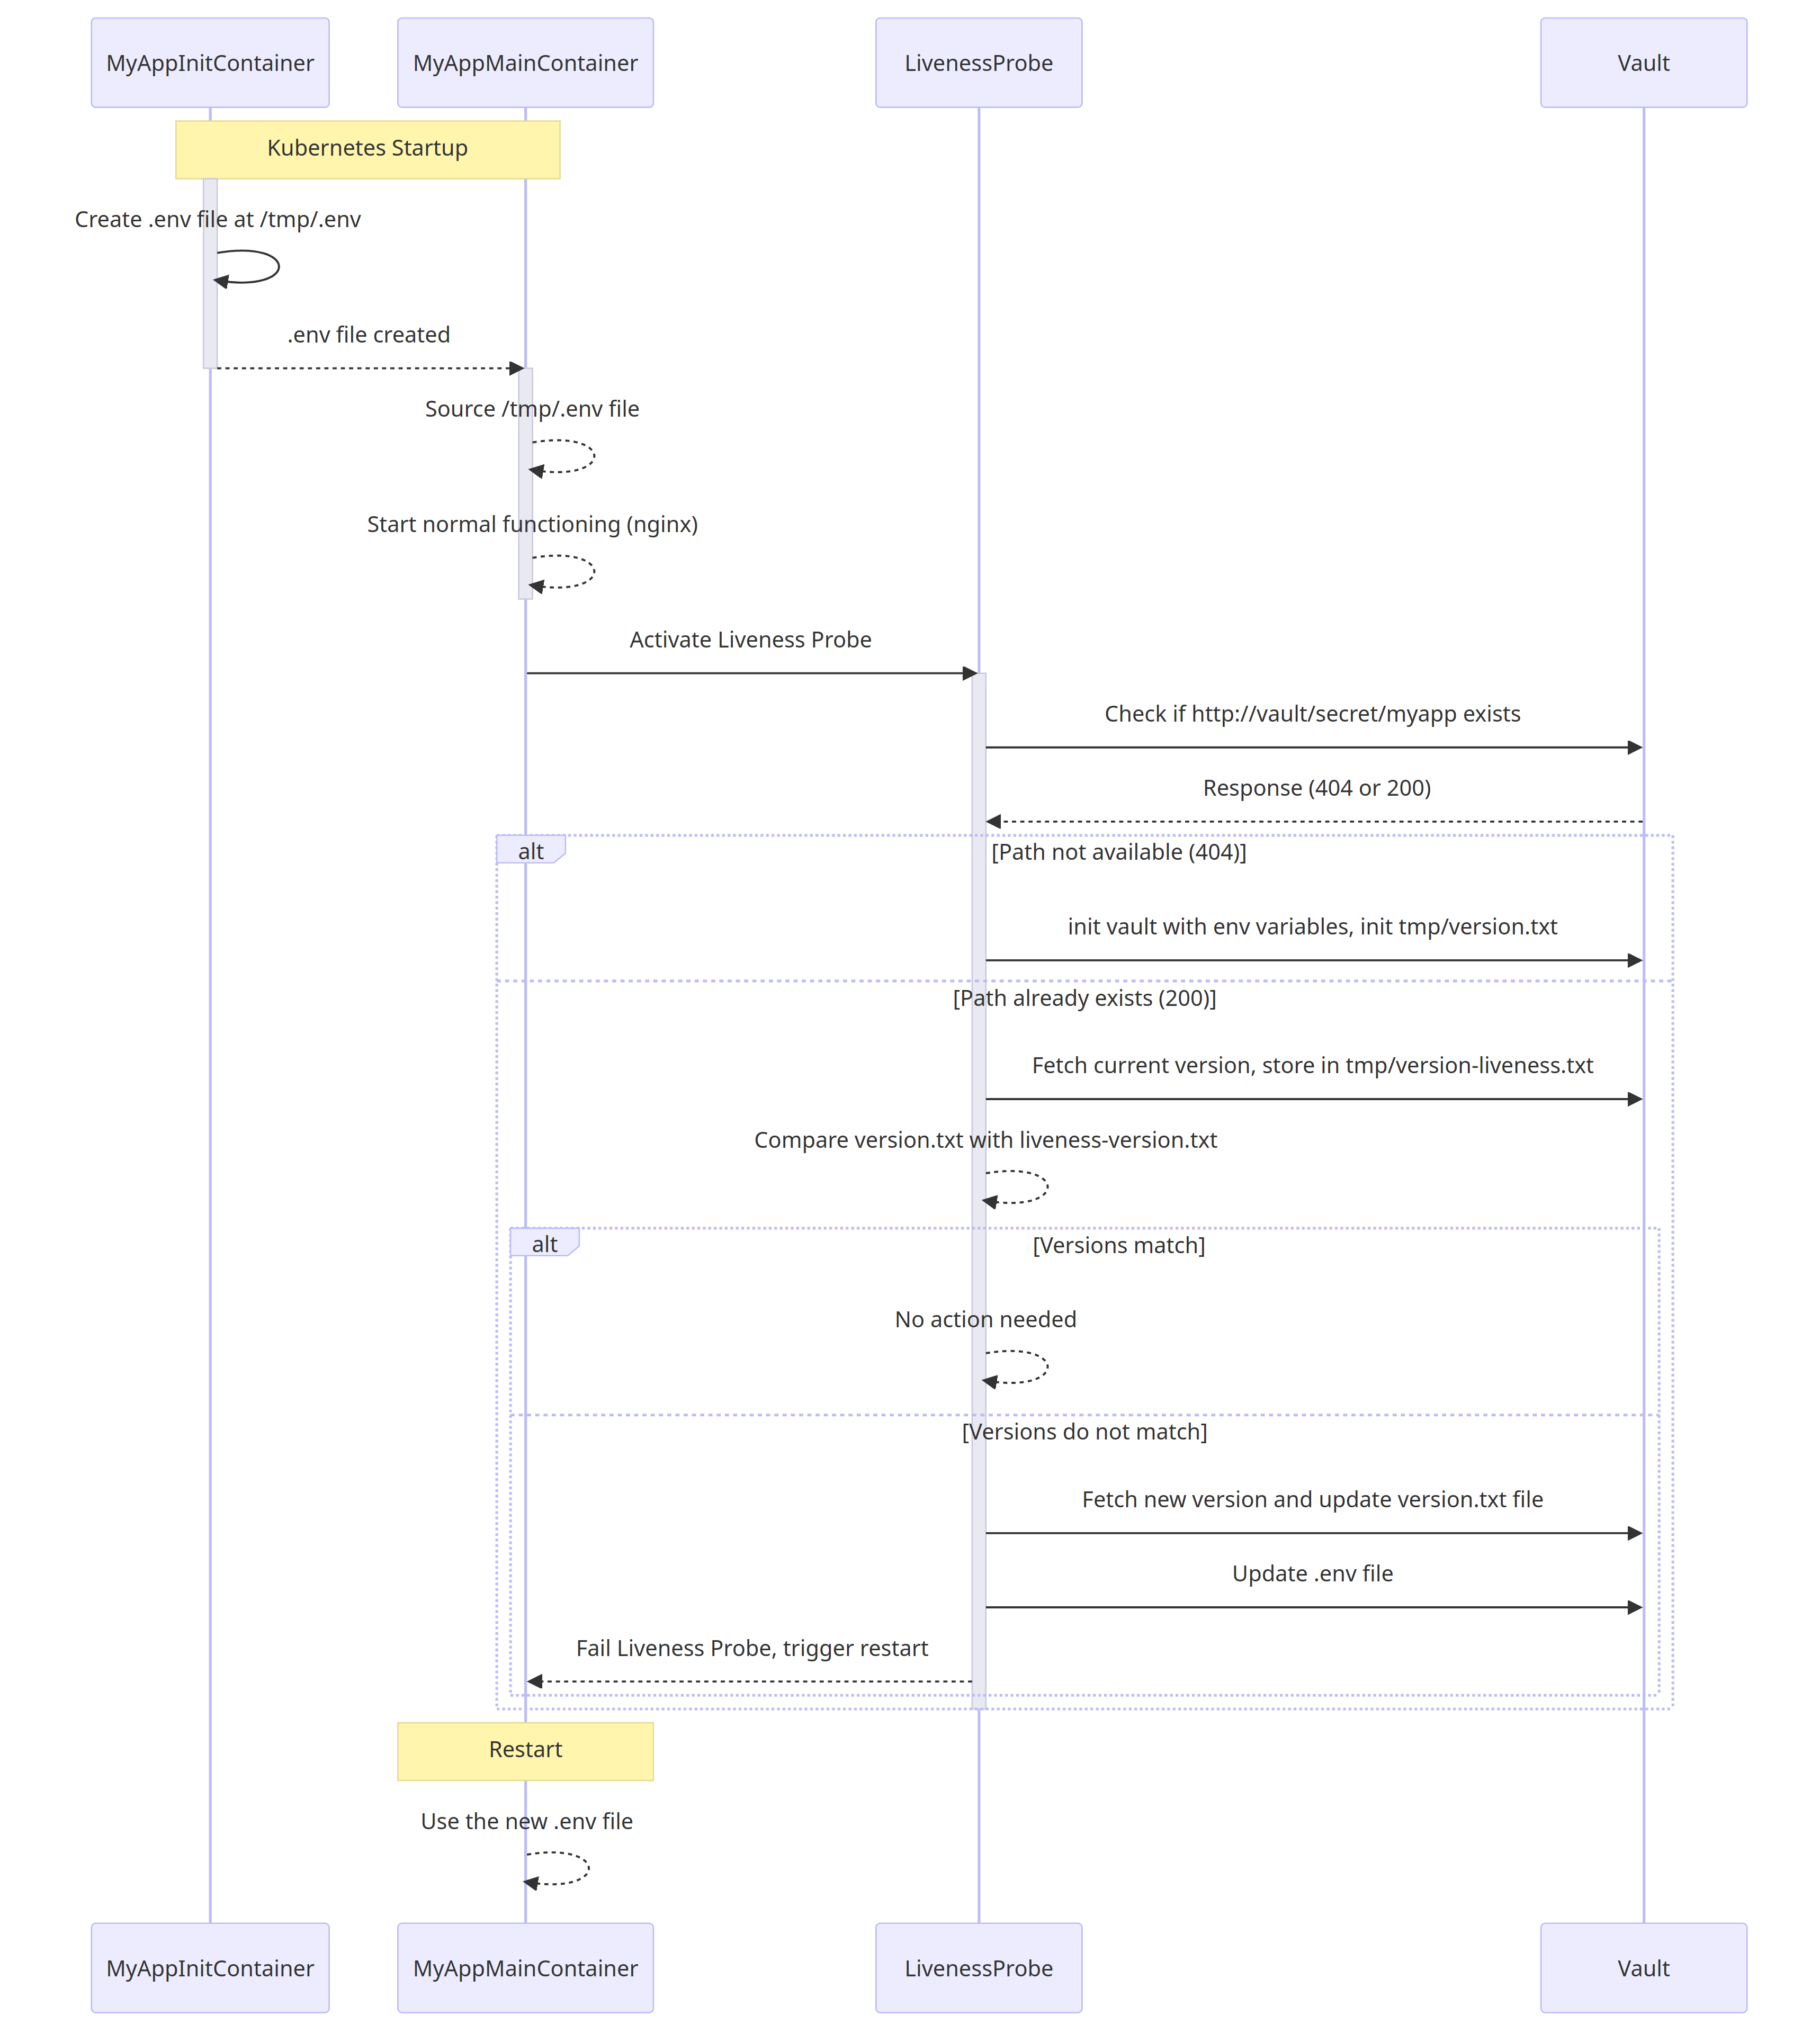
\includegraphics[width=0.8\linewidth]{figures/seq.png}
    \caption{implementation Sequence diagram}
    \label{fig:Sequence diagram}
\end{figure}


\subsection{Working}

The above diagram illustrates the sequence of events within a Kubernetes environment, depicting the initialization and operation of containers, as well as interactions with external services such as Vault for secret management. On start, Kubernetes startup triggers the activation of the \texttt{MyAppInitContainer}, responsible for generating a \texttt{.env} file at \texttt{/tmp/.env}. Subsequently, the \texttt{.env} file is passed to the \texttt{MyAppMainContainer}, which initiates normal application functionality, such as content serving via Nginx. Concurrently, the liveness probe is activated by \texttt{MyAppMainContainer}. The probe then communicates with Vault to verify the availability of a specific path (\texttt{http://vault/secret/myapp}). Depending on the response received, different paths are followed: if the path is absent (\texttt{404}), Vault initializes with environment variables and creates a version file; if present (\texttt{200}), Vault compares the current version with the locally stored version. In case of a version mismatch, Vault updates the version and \texttt{.env} files, leading to the failure of the liveness probe, triggering a restart of \texttt{MyAppMainContainer}. Upon restart, the updated \texttt{.env} file is utilized, ensuring seamless operation with the new environment. (Figure \ref{fig:Sequence diagram}).

\subsection{Kubernetes and Vault Integration}

The script provided facilitates the integration between Kubernetes and HashiCorp Vault. It begins by checking if the \texttt{VAULT\_ENABLE} environment variable is set to "true". If enabled, it proceeds to fetch secrets from Vault using the specified token and address constructed based on environment variables (\texttt{VAULT\_SERVICE\_HOST} and \texttt{VAULT\_SERVICE\_PORT}).

\subsection{Liveness Probe Implementation}

The liveness probe implementation leverages Kubernetes' built-in feature to ensure the health of containerized applications \cite{kubernetes-probes}. Within the script, an HTTP request is made to the specified Vault address to check the availability of secrets. The response status code is evaluated, and actions are taken accordingly. If the secret store is missing (404), it initializes a new Key-Vault secret path. If the token is incorrect (403), it logs an error. Otherwise, it compares the version of the retrieved secrets with the locally stored version. If a mismatch is detected, it updates the environment variables and exports them for the application to use.

\subsection{Deployment Restart Mechanism}

The deployment restart mechanism is triggered conditionally based on the outcome of the liveness probe. If the script detects changes in the environment variables fetched from Vault, it exits with a non-zero status code (1), indicating that a restart is required. This triggers Kubernetes to restart the pod, ensuring that the application picks up the updated environment variables. Conversely, if no changes are detected, the script exits with a zero status code (0), indicating that the environment variables are up to date, and no restart is necessary. This mechanism ensures that the application remains consistent to configuration changes and always uses the latest variables from Vault.
